\documentclass[11pt]{article}

% ---------- Packages ----------
\usepackage[margin=1in]{geometry}
\usepackage{amsmath,amssymb,amsthm}
\usepackage{graphicx}
\usepackage{booktabs}
\usepackage{array}
\usepackage{longtable}
\usepackage{xcolor}
\usepackage[colorlinks=true,linkcolor=blue!50!black,citecolor=blue!50!black,urlcolor=blue!50!black,
  pdftitle={Algorithmic Resolution and Solver-Dependent Observational Geometry in SAT Solution Spaces},
  pdfauthor={Elias De Jesus},
  pdfsubject={Satisfiability, solution-space geometry, Hausdorff resolution, persistent homology, WalkSAT, CDCL},
  pdfkeywords={SAT, satisfiability, solution space geometry, Hausdorff distance, persistent homology, WalkSAT, CDCL, Glucose}
]{hyperref}
\usepackage{natbib}
\usepackage{orcidlink}
\usepackage{caption}
\usepackage{subcaption}
\usepackage{enumitem}
\usepackage{microtype}

% ---------- Theorem environments ----------
\newtheorem{theorem}{Theorem}[section]
\newtheorem{proposition}[theorem]{Proposition}
\newtheorem{corollary}[theorem]{Corollary}
\newtheorem{lemma}[theorem]{Lemma}
\theoremstyle{definition}
\newtheorem{definition}[theorem]{Definition}
\theoremstyle{remark}
\newtheorem{remark}[theorem]{Remark}

% ---------- Macros ----------
\newcommand{\Shat}{S_I}
\newcommand{\Ahat}[1]{A(#1)}
\newcommand{\dH}{d_H}
\newcommand{\dHaus}{d_{\mathrm{Haus}}}
\newcommand{\epshat}{\hat\varepsilon}
\newcommand{\Cov}{\mathrm{Cov}}

\title{\textbf{Algorithmic Resolution and Solver-Dependent Observational Geometry in SAT Solution Spaces}}
\author{
Elias De Jesus\,\orcidlink{0009-0007-0190-9143} \\
\small Independent Researcher \\
\small ORCID: \href{https://orcid.org/0009-0007-0190-9143}{0009-0007-0190-9143}
}
\date{September 2026 \\ \small Draft V2 --- supersedes and corrects the January 2026 preprint \\ \small \emph{``Algorithmic Resolution and Geometric Distinguishability in SAT Solution Spaces''}}

\begin{document}

\maketitle

\begin{abstract}
\noindent
The solution space of a satisfiability instance is usually characterized not directly but through the subset of solutions an algorithm happens to find. We formalize this distinction by separating the intrinsic solution space $\Shat$ from an algorithm's observed subset $\Ahat{I} \subseteq \Shat$, and define the empirical resolution $\epshat(A,I) = \max_{x \in \Shat} \min_{y \in \Ahat{I}} \dH(x,y)$, which for nonempty $\Ahat{I}$ is exactly the Hausdorff distance $\dHaus(\Ahat{I}, \Shat)$ --- a standard quantity, not a new one. Standard Rips-complex persistence stability, specialized here to zero-dimensional homology, bounds how far observed connectivity can drift from true connectivity as a function of $\epshat$; we further show this bound's constant is sharp, including in the discrete Hamming cube. We prove coverage and resolution are logically independent via explicit constructions. Empirically, two structurally different SAT solvers --- WalkSAT and a CDCL solver (Glucose3) --- each show statistically significant, held-out, non-circular prediction of their own eventual blind zones from pre-reveal search dynamics (AUROC $0.658$ and $0.667$ respectively). Our central result: on $349$ paired held-out instances, at matched coverage on the identical solution space, WalkSAT achieves significantly better resolution ($\epshat$; paired $p=5.1\times10^{-38}$) while showing $11.6\times$ (95\% CI $[9.6,13.3]$) greater apparent fragmentation than CDCL. Neither solver dominates; each preserves a different aspect of the true geometry. We report this as a direct empirical instance of the coverage/resolution independence we prove abstractly, and explicitly retract an initially promising but ultimately confounded cross-solver predictive-transfer finding.
\end{abstract}

\noindent\textbf{Status:} Research manuscript, September 2026. Not peer reviewed.

\tableofcontents

% =====================================================================
\section{Introduction}
% =====================================================================

A satisfiability solver is typically asked one question --- is $I$ satisfiable? --- and, if the answer is yes, may return one, several, or many satisfying assignments. When a research question concerns the \emph{structure} of the solution space itself (how solutions cluster, how many distinct regions exist, how far apart they sit), that structure is almost never observed directly. It is inferred from whatever subset of solutions the solver happened to produce, under whatever budget it was given, using whatever search strategy it uses internally.

This creates an identification problem that is easy to state and easy to overlook: a structural claim about ``the solution space of $I$'' is, in practice, a claim about $\Ahat{I}$, the specific finite subset an algorithm $A$ returned --- not about $\Shat \subseteq \{0,1\}^n$, the full set of satisfying assignments. The two can diverge in ways that are not obvious from summary statistics alone. Knowing that an algorithm found, say, 30\% of all solutions does not by itself say whether the missing 70\% is scattered evenly through the space or concentrated in one geometrically remote region; it does not say whether the found solutions form a single connected structure or several apparently disconnected ones, and if the latter, whether that fragmentation reflects the true geometry of $\Shat$ or is an artifact of which solutions happened to be found.

This paper develops a framework for making that identification problem precise, and reports what happens when the framework is applied to two structurally different SAT-solving paradigms --- stochastic local search (WalkSAT) and conflict-driven clause learning (CDCL, via Glucose3) --- on the same random 3-SAT instances.

\subsection{Three distinct quantities}

For an algorithm $A$ observing instance $I$, we distinguish:

\begin{enumerate}[label=(\arabic*)]
\item \textbf{Coverage}: $\Cov(A,I) = |\Ahat{I}| / |\Shat|$ --- what fraction of the true solution set was found.
\item \textbf{Geometric resolution}: $\epshat(A,I)$ --- how far, in Hamming distance, the \emph{worst-represented} true solution sits from the nearest found solution. This is the covering radius of $\Ahat{I}$ relative to $\Shat$, and (Section~\ref{sec:preliminaries}) is exactly the Hausdorff distance between the two sets.
\item \textbf{Connectivity fidelity}: whether the connected-component structure of $\Ahat{I}$, at any given Hamming-distance threshold, matches that of $\Shat$ at the same threshold --- or whether it appears more fragmented, or less, than the truth.
\end{enumerate}

The central question this paper answers empirically: \emph{can two algorithms, observing comparable fractions of the same solution space, nevertheless reveal systematically different geometry?} The answer is yes, and the way in which it is yes is itself informative: on $349$ paired held-out instances, at matched coverage, WalkSAT and a CDCL solver trade off in \emph{opposite directions} on resolution and connectivity fidelity. Neither diagnostic alone characterizes ``how faithfully'' a solver represents $\Shat$; both are necessary, and they are not redundant.

This paper is a substantial revision of a January 2026 preprint under the same general topic. That preprint's central mathematical claim --- a universal distinguishability threshold at $\varepsilon = d/2$ in arbitrary metric spaces --- is false as stated (Section~\ref{sec:hamming-ball} corrects it) and its main quantity, ``algorithmic resolution,'' is a standard Hausdorff-distance construction under new terminology, not a new mathematical object (Section~\ref{sec:preliminaries}). Its empirical evidence for predictable solver blind zones relied on a sampler deliberately biased toward the feature used to predict it, which is close to circular (Section~\ref{sec:cross-solver}). We do not repair the January preprint; we replace its architecture with one built from correctly attributed mathematics and non-circular, freeze-before-reveal experiments, validated across two solver paradigms and audited for the confounds that undermined an initially promising cross-solver finding (Section~\ref{sec:cross-solver}).

\subsection{Contributions}

\begin{enumerate}
\item A clean separation between the intrinsic geometry of a SAT solution space and the algorithm-dependent geometry of what is actually observed, formalized via $\Shat$, $\Ahat{I}$, and three logically independent diagnostics (coverage, resolution, connectivity fidelity).
\item Correct attribution of the covering-radius/Hausdorff-distance identity and the connectivity-recovery stability bound this framework relies on --- both standard, neither claimed as new --- together with one independently verified original result: the recovery bound's constant is sharp, including a construction realized directly in the Hamming cube.
\item A rigorous demonstration, via explicit constructions, that coverage and geometric resolution are logically independent: neither bounds the other without further assumptions on the solution space's geometry.
\item Non-circular, freeze-before-reveal, anti-leakage-verified evidence that both WalkSAT and CDCL search dynamics carry statistically significant held-out information about their own eventual blind zones (AUROC $0.658$ and $0.667$).
\item The paper's central empirical result: at matched coverage, on the same solution space, WalkSAT and CDCL trade off oppositely on resolution and connectivity fidelity --- a direct, real-solver realization of the logical independence proved in Contribution 3.
\item A fully reported, audited negative result: an initially observed cross-solver predictive-transfer asymmetry does not survive confound control and is retracted rather than presented as a finding.
\end{enumerate}

% =====================================================================
\section{Related Work}
% =====================================================================

Random-3-SAT solution-space geometry --- clustering, freezing, the appearance of well-separated regions before the satisfiability threshold --- is established territory \citep{mezard2002analytic,achlioptas2006solution}. Non-uniformity of local-search and DPLL/CDCL-derived samples relative to the true solution distribution is also well documented, motivating an entire line of work on near-uniform SAT sampling via universal hashing \citep{chakraborty2015constrained}. This paper does not contest that solver sampling bias exists; it asks a different, geometric question --- not \emph{whether} a sampler is biased, but \emph{how the specific geometric shape of that bias, measured via covering radius and connectivity, differs between solver paradigms observing the same instance.}

The mathematical machinery --- Hausdorff-distance stability of Vietoris--Rips persistent homology --- is due to \citet{chazal2014persistence} at the level of bottleneck distance between full persistence diagrams. The sharper, asymmetric, zero-dimensional specialization this paper uses --- exploiting that our observed set is literally a subset of the true set, not merely a nearby unrelated point cloud --- is a direct corollary of \citeauthor{harker2019comparison}'s interleaving-based comparison framework \citep{harker2019comparison}, Proposition 5.6(i). We state this attribution explicitly in Section~\ref{sec:stability} rather than presenting the bound as original. Early function-based diagram stability is due to \citet{cohensteiner2007stability}; a more general asymmetric, density-augmented (2-parameter) variant is given by \citet{blumberglesnick2020stability}, in a different setting than the one used here (Section~\ref{sec:stability}). Classical local-search noise strategies and the DPLL algorithm underlying much of modern CDCL are due to \citet{selman1994noise} and \citet{davis1962machine} respectively.

% =====================================================================
\section{Preliminaries}
\label{sec:preliminaries}
% =====================================================================

\begin{definition}[SAT instance and solution space]
A Boolean satisfiability instance $I$ over $n$ variables is a formula in conjunctive normal form; its solution space is $\Shat = \{x \in \{0,1\}^n : I(x) = \mathrm{true}\}$.
\end{definition}

\begin{definition}[Hamming metric]
$\dH(x,y) = |\{i : x_i \neq y_i\}|$; $(\{0,1\}^n, \dH)$ is a metric space.
\end{definition}

\begin{definition}[Observed set and blind zone]
For algorithm $A$ run on $I$, $\Ahat{I} \subseteq \Shat$ is the set of solutions returned within its budget; $M_A(I) = \Shat \setminus \Ahat{I}$ is the blind zone.
\end{definition}

\begin{definition}[Coverage]
$\Cov(A,I) = |\Ahat{I}| / |\Shat|$.
\end{definition}

\begin{definition}[Empirical resolution]
\label{def:epshat}
\[
\epshat(A,I) = \max_{x \in \Shat} \min_{y \in \Ahat{I}} \dH(x,y), \qquad \Ahat{I} \neq \emptyset.
\]
\end{definition}

\begin{proposition}[Standard metric fact, not new]
\label{prop:hausdorff}
For nonempty $\Ahat{I} \subseteq \Shat$,
\[
\epshat(A,I) = \dHaus(\Ahat{I}, \Shat).
\]
\end{proposition}

\begin{proof}
$\epshat(A,I)$ is by definition the directed Hausdorff distance $\vec d(\Shat, \Ahat{I})$. The reverse direction $\vec d(\Ahat{I}, \Shat) = \max_{y \in \Ahat{I}} \min_{x \in \Shat} \dH(y,x) = 0$, since every $y \in \Ahat{I}$ is itself in $\Shat$ at distance $0$ (using $\Ahat{I} \subseteq \Shat$). The symmetric Hausdorff distance is the max of the two directed distances, hence equals $\epshat(A,I)$.
\end{proof}

We retain the domain-facing name ``empirical resolution'' for $\epshat$ --- it usefully signals the interpretation (a solver's effective measurement precision) to a SAT audience --- but state Proposition~\ref{prop:hausdorff} first and explicitly: the underlying object is textbook computational geometry, not a contribution of this paper.

\begin{remark}[The $\Ahat{I}=\emptyset$ case]
This case is handled as a categorical failure flag, not folded into the numeric scale of $\epshat$: the directed Hausdorff distance is $+\infty$ under the standard convention when $\Ahat{I}$ is empty, and reporting it as a bounded sentinel (as the January preprint did) creates a false unconditional inequality, discussed in Appendix~\ref{app:hamming-ball}.
\end{remark}

\begin{table}[htbp]
\centering
\caption{Core quantities used throughout this paper.}
\label{tab:definitions}
\begin{tabular}{@{}p{4cm}p{5.7cm}l@{}}
\toprule
Quantity & Definition & Status \\
\midrule
Coverage & $\Cov(A,I) = |\Ahat{I}|/|\Shat|$ & Standard \\
Empirical resolution & $\epshat(A,I) = \dHaus(\Ahat{I},\Shat)$ & Standard (Hausdorff distance) \\
Blind zone & $M_A(I) = \Shat \setminus \Ahat{I}$ & Standard \\
Cluster spectrum & $C_S(r)$: components of $S$ at threshold $r$ & Standard (0-dim persistence) \\
Observed fragmentation & $C_A(r) - C_S(r)$ at the same $r$ & This paper's diagnostic use \\
\bottomrule
\end{tabular}
\end{table}

% =====================================================================
\section{A Corrected Discrete-Space Result}
\label{sec:hamming-ball}
% =====================================================================

The January preprint's central geometric claim was: in an arbitrary metric space, points at distance $D$ are distinguishable by a measurement of resolution $\varepsilon$ if and only if $\varepsilon < D/2$. This is false in general and specifically false in the Hamming cube. Take $x,y \in \{0,1\}^n$ with $\dH(x,y)=1$ and $\varepsilon=1$: the open ball $B_1(x) = \{z : \dH(x,z)<1\} = \{x\}$ and likewise $B_1(y)=\{y\}$, so the balls are disjoint (the points \emph{are} distinguishable) --- yet $\varepsilon=1 \not< D/2 = 0.5$, contradicting the claimed threshold.

The error traces to an implicit midpoint assumption: the proof's forward direction requires a point exactly at distance $D/2$ from both $x$ and $y$, which exists in continuous, geodesic metric spaces but not in the integer-valued, discrete Hamming cube whenever $D$ is odd.

\begin{theorem}[Corrected, proved and exhaustively verified]
\label{thm:hamming-ball}
For $x,y \in \{0,1\}^n$ with $\dH(x,y)=D>0$ and real $\varepsilon>0$:
\begin{align}
B_\varepsilon(x) \cap B_\varepsilon(y) = \emptyset &\iff \varepsilon \le \lceil D/2 \rceil \qquad \text{(open balls)}, \\
\bar B_\varepsilon(x) \cap \bar B_\varepsilon(y) = \emptyset &\iff \varepsilon < \lceil D/2 \rceil \qquad \text{(closed balls)}.
\end{align}
\end{theorem}

\begin{proof}[Proof sketch]
The minimum, over $z \in \{0,1\}^n$, of $\max(\dH(x,z), \dH(y,z))$ equals $\lceil D/2 \rceil$ exactly, achieved by splitting the $D$ differing coordinates as evenly as possible; the stated biconditionals follow directly. Full proof in Appendix~\ref{app:hamming-ball}.
\end{proof}

Theorem~\ref{thm:hamming-ball} was exhaustively verified computationally: $45{,}393$ $(n,D,\varepsilon)$ cases, $n=1$--$10$ (exhaustive for $n \le 6$, representative-plus-transitivity-spot-checked for $n=7$--$10$), zero mismatches. This section is brief by design; the theorem is elementary once correctly stated, and this paper's central contribution lies elsewhere (Sections~\ref{sec:coverage-resolution}--\ref{sec:paired-observer}).

% =====================================================================
\section{Coverage and Resolution Are Logically Independent}
\label{sec:coverage-resolution}
% =====================================================================

Neither coverage nor $\epshat$ determines the other without further assumptions on $\Shat$'s geometry. We exhibit two explicit, verified, parameterized families.

\begin{proposition}[Family A --- high coverage, poor resolution]
\label{prop:family-a}
For each $n$, let $S_n = \{0^n\} \cup \{\text{weight-1 vectors}\} \cup \{1^n\}$ ($|S_n|=n+2$) and $A_n = S_n \setminus \{1^n\}$. Then
\[
\Cov(A_n,S_n) = \frac{n+1}{n+2} \to 1, \qquad \epshat(A_n,S_n) = n-1,
\]
so $\epshat/\mathrm{diam} \to 1$ simultaneously --- coverage approaching $1$ and resolution approaching the worst possible value at once.
\end{proposition}

A single omitted point, however rare in relative terms, can be arbitrarily geometrically catastrophic.

\begin{proposition}[Family B --- low coverage, good resolution]
\label{prop:family-b}
For $n=2^m-1$, let $S_n = \{0,1\}^n$ (the full cube) and $A_n$ a perfect binary Hamming code (covering radius exactly $1$, $|A_n| = 2^n/(n+1)$). Then
\[
\Cov(A_n,S_n) = \frac{1}{n+1} \to 0, \qquad \epshat(A_n,S_n) = 1 \ \text{(constant)}.
\]
\end{proposition}

Verified exactly (via syndrome decoding, not brute force) up to $n=63$ ($|A_n| = 2^{57}$). These are standard coding-theoretic ingredients (perfect codes, covering radius) recombined into an explicit demonstration \citep{cohen1997covering}; the underlying facts are not new. What Propositions~\ref{prop:family-a} and~\ref{prop:family-b} jointly establish --- that no deterministic inequality can relate $\Cov(A,I)$ and $\epshat(A,I)$ without further structural assumptions on $\Shat$ --- is the theoretical basis for why raw coverage cannot substitute for $\epshat$, or vice versa, as a diagnostic of solver fidelity. Section~\ref{sec:paired-observer} shows this abstract, worst-case divergence is realized concretely by real solvers on real instances.

% =====================================================================
\section{Connectivity Fidelity and Its Stability Bound}
\label{sec:stability}
% =====================================================================

For $S \subseteq \{0,1\}^n$ and threshold $r \ge 0$, let $C_S(r)$ denote the number of connected components of the graph on $S$ with an edge between $p,q$ whenever $\dH(p,q) \le r$ --- the zero-dimensional persistence / cluster spectrum of $S$. This function is exactly the connected-component count of the Vietoris--Rips complex of $S$ at scale $r$.

\begin{theorem}[Known result, specialized to $H_0$ --- \citealp{harker2019comparison}, Prop.\ 5.6(i)]
\label{thm:stability}
Let $A \subseteq S$ with $\epshat(A,S) = \varepsilon$. Then:
\begin{enumerate}[label=(\alph*)]
\item \emph{No false merge, zero slack.} If $x,y \in A$ are connected in $A$'s $r$-cluster graph, they are connected in $S$'s $r$-cluster graph.
\item \emph{Guaranteed recovery, $+2\varepsilon$.} If $x,y \in S$ are connected in $S$'s $r$-cluster graph, their nearest-$A$ images are connected in $A$'s $(r+2\varepsilon)$-cluster graph.
\end{enumerate}
\end{theorem}

Part (a) is immediate from $A \subseteq S$ (any chain of points in $A$ is a valid chain in $S$).

We state this attribution carefully because an earlier stage of this project's development mistakenly treated Theorem~\ref{thm:stability} as new. \citeauthor{harker2019comparison}'s Proposition 5.6(i) --- stated for general persistence modules under their $\delta$-approximation hypothesis (word-for-word our $A \subseteq S$, $\delta = \varepsilon$), with their Rips parameter $t$ related to our radius by $r=2t$ --- is, once this convention is tracked, exactly Theorem~\ref{thm:stability}, generalized to all homological dimensions. Restricting to $H_0$ recovers our statement verbatim, including the exact constant $+2\varepsilon$ (full translation in Appendix~\ref{app:harker}). We present it here as a citation-grounded application, not a contribution.

\begin{corollary}
\label{cor:stability}
$C_A(r+2\varepsilon) \le C_S(r)$ for all $r$: any apparent fragmentation in the observed set is guaranteed to resolve once the radius is loosened by $2\varepsilon$.
\end{corollary}

We verified Corollary~\ref{cor:stability} directly against $349$ real SAT solution spaces: zero violations across approximately $7{,}000$ (instance, $r$) checks.

\begin{proposition}[Sharpness --- independently verified, narrow-scope original contribution]
\label{prop:sharpness}
The constant $2$ in Theorem~\ref{thm:stability}(b) cannot be improved. For any $r,\varepsilon \ge 1$, an explicit four-point construction in $\{0,1\}^{r+2\varepsilon}$ --- using three disjoint coordinate blocks to independently realize the worst case on each side of the triangle inequality --- achieves $\dH(a,b) = r+2\varepsilon$ exactly, where $a,b$ are the nearest-$A$ images of two directly $r$-connected points of $S$.
\end{proposition}

Verified across seven $(r,\varepsilon)$ combinations. We did not locate an explicit statement of this sharpness result, in the general metric-space case or the Hamming-cube-specific case, anywhere in the literature searched; we report this as an absence, not as a novelty claim, following our own discipline against inferring novelty from a failed search.

\begin{proposition}[Exact conditions for naive monotonicity]
\label{prop:monotone}
$C_A(r) \ge C_S(r)$ is guaranteed exactly once $r \ge \varepsilon$ (every $x \in S$ then has a directly-connected nearest neighbor in $A$, ruling out under-representation of whole components); this can fail for $r<\varepsilon$, where an entire $S$-component with no representative in $A$ pulls $C_A(r)$ below $C_S(r)$ --- a distinct failure mode from fragmentation.
\end{proposition}

Verified: $877/877$ random-instance checks confirm the $r \ge \varepsilon$ guarantee; an explicit counterexample confirms the failure mode below it (Appendix~\ref{app:harker}).

% =====================================================================
\section{Experimental Design}
\label{sec:experiment}
% =====================================================================

\paragraph{Instances.} $720$ random 3-SAT instances ($360$ train / $360$ test, split by instance), $n \in \{16,18,20\}$, $\alpha \in \{2.5 \text{ (solution-rich)}, 3.5 \text{ (intermediate)}, 4.2 \text{ (near-threshold)}\}$, $40$ instances per $(n,\alpha)$ cell per split, all satisfiable, \textbf{no solution cap} (the January preprint's fixed 500-solution cap was found, in an earlier audit phase, to truncate the true solution set itself at low $\alpha$ for $64$--$100\%$ of instances at $n \ge 18$ --- a confound removed entirely here by exhaustive enumeration).

\paragraph{WalkSAT.} Standard random-walk/greedy local search: $K=150$ independent restarts, $\mathrm{max\_flips}=3000$, noise parameter $p=0.5$.

\paragraph{CDCL.} Glucose3 \citep{audemard2009predicting}, accessed via PySAT \citep{ignatiev2018pysat} --- a genuine, unmodified, competition-grade CDCL solver (VSIDS branching, first-UIP clause learning, LBD-based aggressive restarts), not a homemade DPLL implementation \citep{davis1962machine}. Solution enumeration via native blocking-clause iteration. Since Glucose3 exposes no direct RNG seed, independent runs are obtained via a mathematically exact symmetry of the CNF (uniformly random variable relabeling and clause-order shuffling) combined with randomized initial-phase hints --- confirmed empirically to produce genuinely different search trajectories and discovery orders across seeds. Primary budget: $R=5$ independent permuted runs, $T=8$ solutions enumerated per run, calibrated (on coverage statistics alone, before any predictive result was examined) to give CDCL a coverage level comparable in order of magnitude to WalkSAT's on the same instances.

\paragraph{Freeze-before-reveal protocol.} For every predictive experiment, a Stage-A process sees only the CNF formula and the solver's own trajectory (flips/restarts for WalkSAT; permutation seeds, conflicts/decisions/restarts counters for CDCL) and writes its predictions to disk with a SHA-256 hash and UTC timestamp before any ground-truth enumeration occurs; a separate Stage-B process verifies that hash before revealing $\Shat$. For the CDCL pipeline, this isolation is additionally enforced by a programmatic runtime guard that raises an error if Stage-A code attempts to open any ground-truth-bearing file path --- tested directly to confirm it trips correctly.

\paragraph{Statistical unit.} The SAT instance, never an individual solution (solutions within one instance are highly dependent). All reported metrics are computed per instance first, then aggregated via median and instance-level bootstrap ($5{,}000$ resamples) for confidence intervals, with instance-level permutation tests ($1{,}000$ permutations, label-shuffling within each instance) for significance.

\begin{table}[htbp]
\centering
\caption{Experimental configuration summary.}
\label{tab:config}
\begin{tabular}{@{}ll@{}}
\toprule
Parameter & Value \\
\midrule
Instances & 720 (360 train / 360 test), split by instance \\
$n$ & $\{16, 18, 20\}$ \\
$\alpha$ regimes & 2.5 (solution-rich), 3.5 (intermediate), 4.2 (near-threshold) \\
Instances per $(n,\alpha)$ cell per split & 40 \\
Solution cap & None \\
WalkSAT restarts $K$ & 150 \\
WalkSAT max flips & 3000 \\
WalkSAT noise $p$ & 0.5 \\
CDCL solver & Glucose3 (PySAT 1.9.dev15) \\
CDCL randomization & Variable/clause permutation + phase hints \\
CDCL budget & $R=5$ permuted runs $\times$ $T=8$ solutions/run \\
$\rho$ (miss-radius) & 1.0 (frozen from train split) \\
CI method & Instance-level bootstrap, 5{,}000 resamples \\
Significance test & Instance-level permutation test, 1{,}000 permutations \\
\bottomrule
\end{tabular}
\end{table}

% =====================================================================
\section{Prospective Blind-Zone Prediction}
\label{sec:prediction}
% =====================================================================

For each solver, a risk score computed \emph{only} from pre-reveal search dynamics is tested against the retrospective blind zone after reveal.

\paragraph{WalkSAT: \texttt{risk\_basin}.} For each found solution $y$, $\mathrm{basin}(y)$ counts how many of the $K=150$ restarts converge to $y$; low basin count is hypothesized to predict higher local miss risk.

\paragraph{CDCL: \texttt{risk\_cdcl\_recurrence}.} No restart concept exists for blocking-clause enumeration; the structural analogue is $\mathrm{recurrence}(y)$, the number of independent permuted search orderings (out of $R=5$) that rediscover $y$.

\begin{table}[htbp]
\centering
\caption{Held-out blind-zone prediction, test split, touched once. Baselines and failed predictors reported in full; see Appendix~\ref{app:stratification} for stratified breakdowns.}
\label{tab:prediction}
\footnotesize
\begin{tabular}{@{}llccc@{}}
\toprule
Solver & Predictor & Median AUROC [95\% CI] & Median Spearman & Permutation $p$ \\
\midrule
WalkSAT & \texttt{risk\_basin} & \textbf{0.658} [0.636, 0.685] & 0.252 & 0.000999 \\
WalkSAT & \texttt{risk\_disc\_flips} (failed) & 0.407 & $-0.160$ & --- \\
WalkSAT & Hamming weight & 0.519 & 0.025 & --- \\
WalkSAT & random (sanity) & 0.504 & 0.016 & 0.347 \\
\addlinespace
CDCL & \texttt{risk\_cdcl\_recurrence} & \textbf{0.667} [0.647, 0.700] & 0.346 & 0.000999 \\
CDCL & \texttt{conflicts\_to\_discovery} (failed) & 0.471 & $-0.043$ & --- \\
CDCL & Hamming weight & 0.492 & $-0.011$ & --- \\
CDCL & random (sanity) & 0.481 & $-0.001$ & 0.934 \\
\bottomrule
\end{tabular}
\end{table}

Both solvers show a genuine, comparably sized effect (overlapping confidence intervals; Table~\ref{tab:prediction}), robust to stratification by SAT regime, $n$, and $|\Shat|$ tercile in both cases (Appendix~\ref{app:stratification}). We report the failed predictors --- flip/conflict-count-based ``harder discovery predicts higher risk'' did not hold for either solver --- as informative negative sub-results, not as post-hoc-rescued findings. \textbf{We claim only that each solver's own dynamics predict its own blind zone}; cross-solver transfer is addressed, and rejected, next.

% =====================================================================
\section{A Retracted Cross-Solver Finding}
\label{sec:cross-solver}
% =====================================================================

A natural follow-up question is whether one solver's risk score predicts the \emph{other} solver's blind zone --- evidence, if it held up, of a shared underlying accessibility structure. Raw cross-prediction showed an asymmetry: \texttt{risk\_basin} (WalkSAT) predicted CDCL's blind zone at AUROC $0.625$; \texttt{risk\_cdcl\_recurrence} (CDCL) predicted WalkSAT's blind zone at only $0.526$.

This did not survive confound analysis, and we report it as retracted rather than as a finding. Three independent methods converge:
\begin{enumerate}
\item A joint model using only generic confounds (Hamming weight, local density, distance to the other solver's set, instance size, coverage, $\epshat$, regime) already reaches AUROC $0.946$ (or $0.756$ excluding the single strongest, most tautology-adjacent confound), and adding the solver-specific risk score improves discrimination by approximately zero in both directions.
\item Residualizing each risk score against the same confounds leaves a residual with no reliable within-instance predictive power ($0.441$ and $0.589$ median per-instance AUROC, both statistically indistinguishable from noise).
\item Restricting to instances where the two solvers' coverage levels are matched shrinks the WalkSAT$\to$CDCL figure from $0.625$ to $0.556$.
\end{enumerate}
The dominant confound is a coverage-calibration mismatch: CDCL's tested budget gave it systematically lower mean coverage than WalkSAT on the same instances, mechanically inflating the apparent transfer.

A specific alternative hypothesis --- that a risk score identifies solutions that are difficult to find by \emph{any} method (a solver-agnostic rarity signal) --- was tested directly and also not supported: while pooled correlations between a risk score and joint-discoverability-by-both-solvers are large, the within-instance ranking ability is at or near chance ($0.533$, $0.500$), indicating the pooled correlation is a between-instance artifact of shared confounds rather than a genuine solution-level sensing capability.

We explicitly do not use, and found no evidence supporting, dynamical-systems language (``conjugacy,'' ``semiconjugacy'') for any relationship between the two solvers: no state-space map between their respective search dynamics was ever constructed, and the predictive relationship the terminology would have decorated is itself the confounded finding just retracted.

% =====================================================================
\section{The Paired Observer Effect}
\label{sec:paired-observer}
% =====================================================================

This is the paper's central empirical result. For all $349$ held-out test instances with both solvers' observed sets nonempty, we compare $A_W(I)$ and $A_C(I)$ against the identical, freshly re-enumerated $\Shat$, at each solver's standard experimental budget (Section~\ref{sec:experiment}) --- no post-hoc budget tuning to produce this result.

\begin{figure}[htbp]
\centering
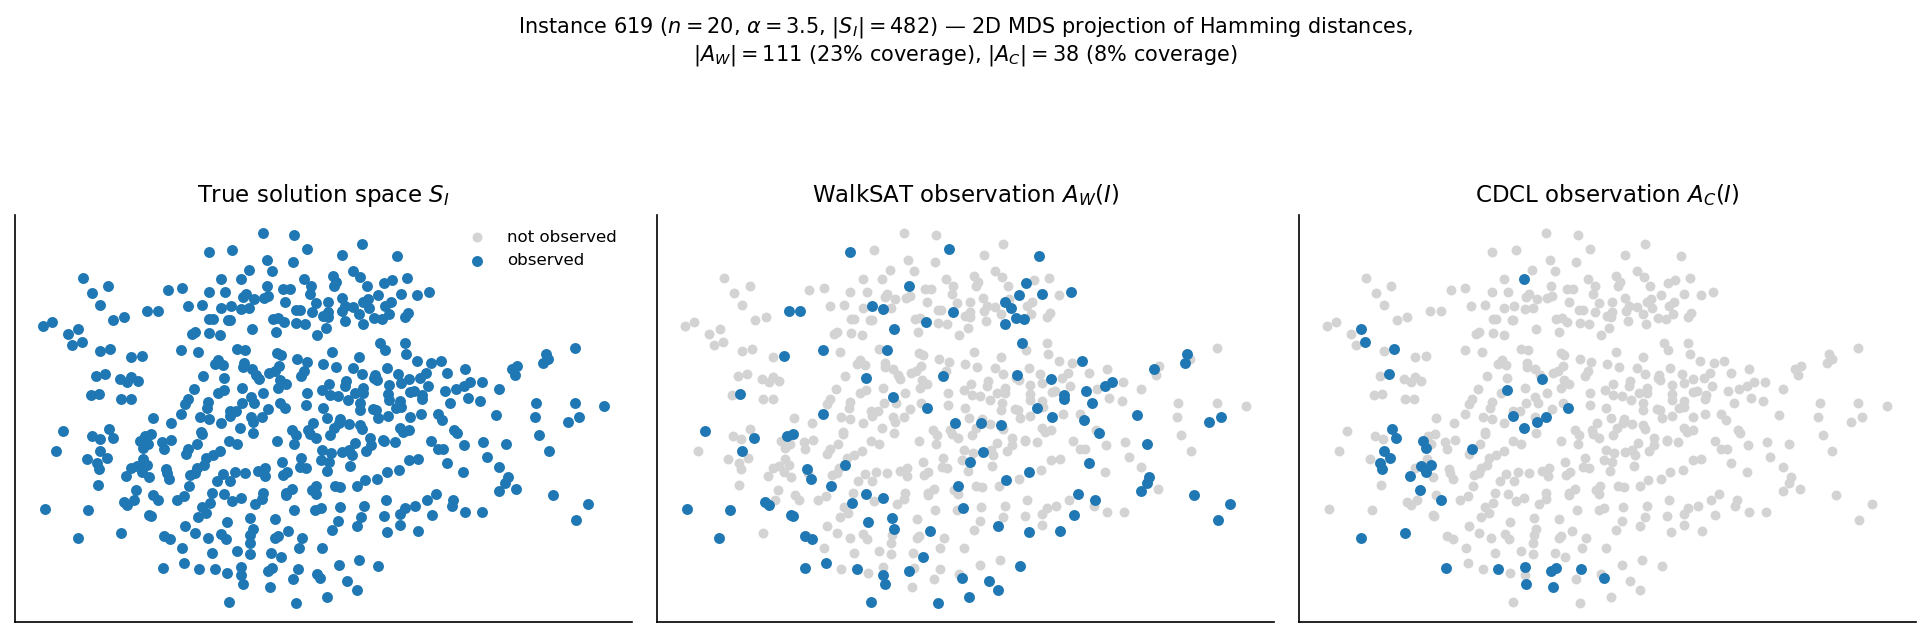
\includegraphics[width=0.95\textwidth]{figures/figure1_schematic.png}
\caption{Conceptual illustration on a real instance ($n{=}20$, $\alpha{=}3.5$, $|\Shat|{=}482$; the same instance used throughout the paired budget-trajectory analysis): 2D MDS projection of pairwise Hamming distances within $\Shat$, with the true set (left) against WalkSAT's (center) and CDCL's (right) observed subsets at their standard budgets. Coverage differs between the two solvers in this particular illustration (23\% vs.\ 8\%); the matched-coverage statistical comparison is given in Figures~\ref{fig:fragmentation} and~\ref{fig:epsilon}.}
\label{fig:schematic}
\end{figure}

\begin{figure}[htbp]
\centering
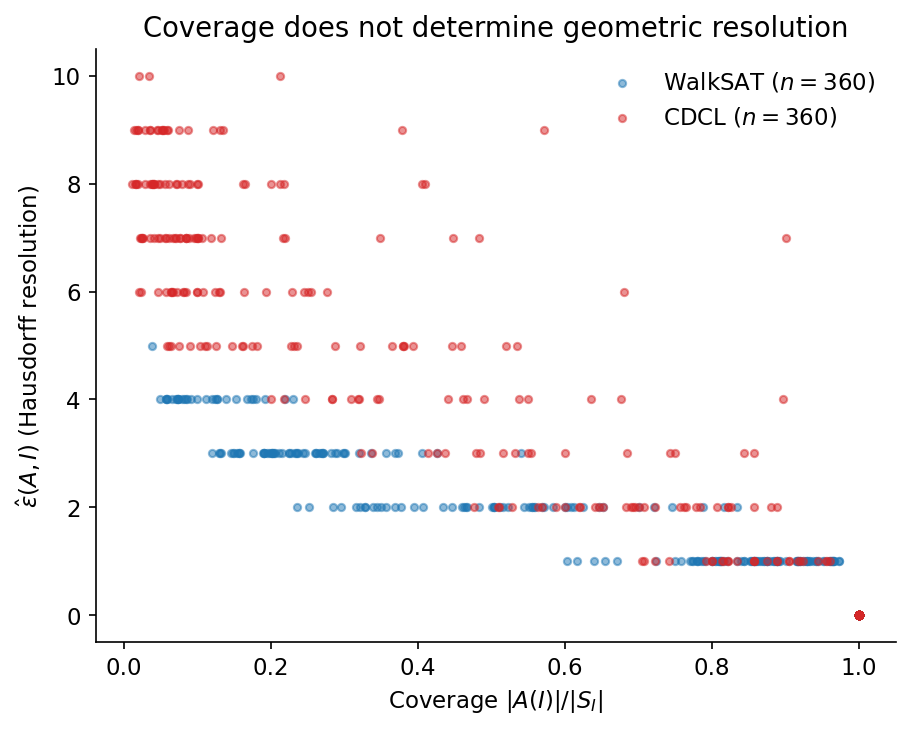
\includegraphics[width=0.7\textwidth]{figures/figure2_coverage_vs_resolution.png}
\caption{Coverage does not determine $\epshat$: all $360$ test instances, both solvers. Points span a wide range of $\epshat$ at any fixed coverage level, consistent with Propositions~\ref{prop:family-a}--\ref{prop:family-b}.}
\label{fig:coverage-resolution}
\end{figure}

\paragraph{Fragmentation.} At fixed radius $r=1$, WalkSAT's excess-component count ($C_{A_W}(1) - C_S(1)$) is a median $11.6\times$ (95\% CI $[9.6, 13.3]$) larger than CDCL's, paired Wilcoxon $p=5.2\times10^{-31}$. The effect holds in every regime, every $n$, every coverage band tested, and --- critically --- survives restricting to the $160$ instances where the two solvers' coverage levels are matched within $10$ percentage points (paired $p=2.4\times10^{-7}$; Figure~\ref{fig:fragmentation}).

\begin{figure}[htbp]
\centering
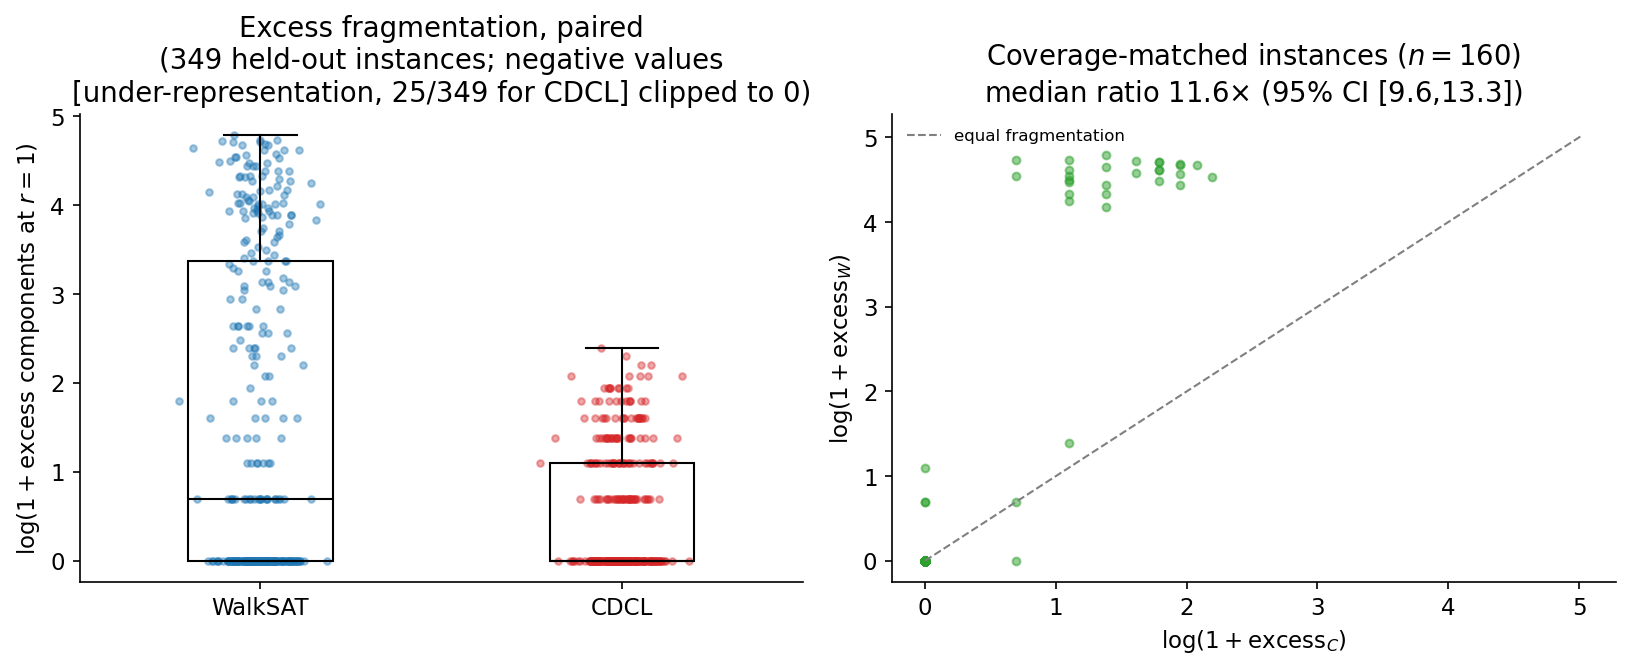
\includegraphics[width=0.95\textwidth]{figures/figure4_fragmentation_matched_coverage.png}
\caption{Excess fragmentation, WalkSAT vs.\ CDCL, paired on the same $349$ instances (left; negative values --- under-representation, a distinct phenomenon per Proposition~\ref{prop:monotone}, occurring for $25/349$ CDCL instances --- clipped to zero for this visualization) and restricted to the $160$ coverage-matched instances (right; every point lies above the equal-fragmentation line).}
\label{fig:fragmentation}
\end{figure}

\paragraph{Resolution.} On the same $349$ paired instances, WalkSAT achieves significantly \emph{better} $\epshat$ than CDCL: mean $1.413$ versus $3.516$, paired Wilcoxon $p=5.1\times10^{-38}$, surviving the same coverage-matched restriction ($p=2.5\times10^{-8}$; Figure~\ref{fig:epsilon}).

\begin{figure}[htbp]
\centering
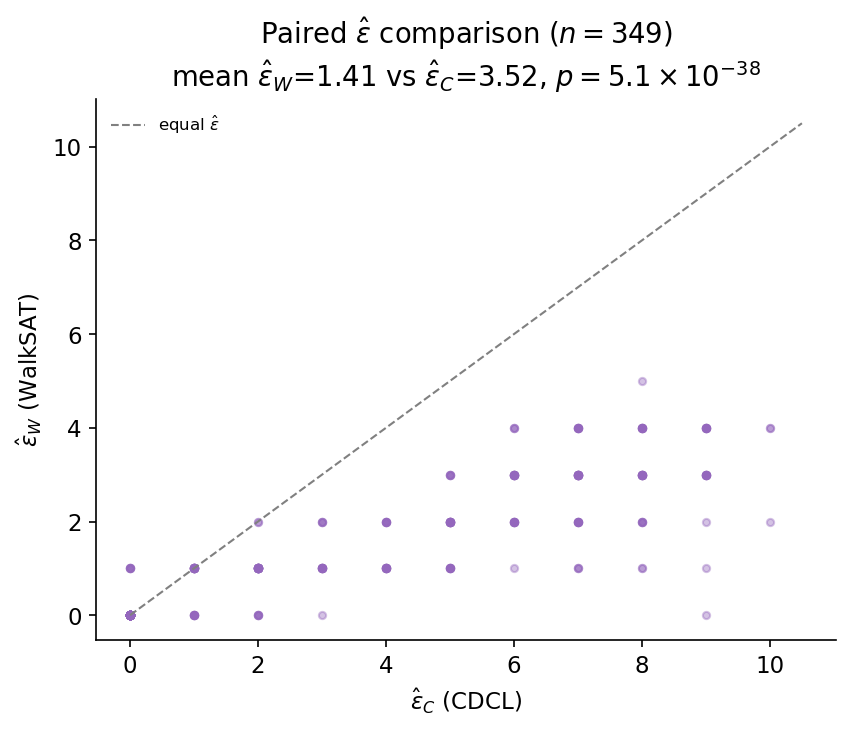
\includegraphics[width=0.6\textwidth]{figures/figure5_epsilon_reversal.png}
\caption{Paired $\epshat$ comparison, same $349$ instances as Figure~\ref{fig:fragmentation}. WalkSAT achieves smaller (better) $\epshat$ despite showing dramatically worse fragmentation --- the two diagnostics move in opposite directions.}
\label{fig:epsilon}
\end{figure}

\paragraph{The trade-off is the finding.} WalkSAT wins on resolution and loses badly on connectivity fidelity; CDCL does the reverse. Neither solver is geometrically superior in an unqualified sense --- each better preserves a different, logically independent aspect of $\Shat$'s true geometry (Section~\ref{sec:coverage-resolution}), and this is not a contradiction of the stability bound in Section~\ref{sec:stability}: that bound is a one-directional worst-case guarantee (small $\epshat$ bounds \emph{how much} distortion is possible, not that distortion must be small), and CDCL's larger $\epshat$ does not violate it --- it simply operates further from the bound's tightest regime while still, empirically, showing far less realized distortion in practice.

\begin{figure}[htbp]
\centering
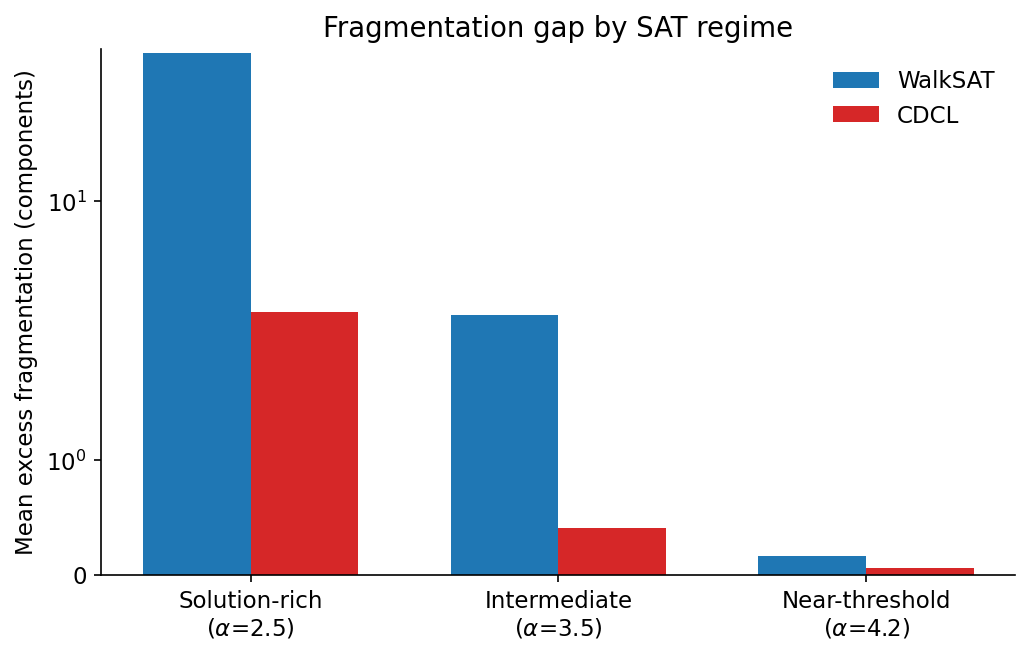
\includegraphics[width=0.85\textwidth]{figures/figure6_regime_dependence.png}
\caption{The fragmentation gap by SAT regime (349 instances). Note-worthy: log scale on the vertical axis given the wide dynamic range.}
\label{fig:regime}
\end{figure}

\begin{table}[htbp]
\centering
\caption{Matched-coverage WalkSAT/CDCL comparison, 349 paired instances.}
\label{tab:matched}
\footnotesize
\begin{tabular}{@{}lccc@{}}
\toprule
Diagnostic & WalkSAT & CDCL & Paired test \\
\midrule
Mean excess fragmentation ($r=1$) & 18.96 & 1.16 & $p=5.2\times10^{-31}$ \\
Median fragmentation ratio (W/C) & \multicolumn{2}{c}{11.6$\times$ [9.6, 13.3] 95\% CI} & survives coverage-matching \\
Mean $\epshat$ & 1.413 & 3.516 & $p=5.1\times10^{-38}$ \\
Fraction fragmented (excess $>0$) & 50.4\% & 42.4\% & --- \\
\bottomrule
\end{tabular}
\end{table}

This result is, to our knowledge, the first demonstration that the abstract coverage/resolution independence proved in Section~\ref{sec:coverage-resolution} --- established there via hand-built extremal point-set constructions --- is realized ``in the wild'' by two real, unmodified, off-the-shelf SAT solvers on real random-3-SAT instances, rather than only as a worst-case existence proof.

% =====================================================================
\section{Discussion and Limitations}
% =====================================================================

\paragraph{What this paper establishes.} A corrected, exact discrete distinguishability theorem; a correctly attributed (not novel) connectivity-stability bound with one independently verified sharpness result; a proof that coverage and resolution are logically independent; non-circular held-out evidence that two solver paradigms each predict their own blind zones; and --- the central contribution --- direct empirical evidence that solver identity materially and \emph{oppositely} shapes two geometric diagnostics of the same solution space at matched coverage.

\paragraph{What this paper does not establish.} No claim is made about computational complexity, hardness characterization, or which solver paradigm is preferable for any practical purpose. No portfolio-performance claim is made beyond the narrow observation that the union of the two solvers' found sets improves $\epshat$ on a real but modest ($15.6\%$) minority of instances (Appendix~\ref{app:portfolio}) --- this is reported as a geometric observation, not an engineering recommendation. No dynamical or causal relationship between the two solvers is claimed.

\paragraph{Scope.} The paired observer effect (Section~\ref{sec:paired-observer}) is established for two specific, carefully audited implementations --- this WalkSAT configuration and Glucose3 specifically --- on random 3-SAT with $n \le 20$ (the ceiling imposed by exhaustive ground-truth enumeration). Whether the resolution/connectivity trade-off generalizes across local-search implementations, across CDCL solvers, to structured or larger instances, or to other constraint-satisfaction domains, is an open question this paper does not address.

\paragraph{Coverage/resolution near-redundancy, and why it is not the whole story.} For WalkSAT alone, coverage and $\epshat$ are empirically almost perfectly anti-correlated across our instance ensemble ($\rho=-0.975$) --- in that narrow sense $\epshat$ adds little practical information beyond coverage \emph{for a single solver}. Section~\ref{sec:paired-observer}'s cross-solver result shows this near-redundancy is not fundamental: introducing a second solver paradigm on the identical instances reveals the two diagnostics diverging sharply and reproducibly.

% =====================================================================
\appendix
% =====================================================================

\section{Hamming-Ball Theorem: Full Proof and Verification}
\label{app:hamming-ball}

\begin{proof}[Full proof of Theorem~\ref{thm:hamming-ball}]
Let $D = \dH(x,y)$. For any $z \in \{0,1\}^n$, write $a = \dH(x,z)$, $b=\dH(y,z)$. By the triangle inequality $a+b \ge D$, so $\max(a,b) \ge D/2$; since $a,b$ are integers, $\max(a,b) \ge \lceil D/2 \rceil$. This bound is achieved: partition the $D$ coordinates on which $x,y$ differ into a block of size $\lceil D/2 \rceil$ and a block of size $\lfloor D/2 \rfloor$; let $z^*$ agree with $y$ on the first block and with $x$ on the second (and with both, trivially, elsewhere). Then $\dH(x,z^*) = \lceil D/2 \rceil$ and $\dH(y,z^*) = \lfloor D/2 \rfloor$, so $\max(\dH(x,z^*),\dH(y,z^*)) = \lceil D/2 \rceil$. Hence
\[
\min_{z \in \{0,1\}^n} \max(\dH(x,z),\dH(y,z)) = \lceil D/2 \rceil.
\]
For open balls, $B_\varepsilon(x)\cap B_\varepsilon(y) \neq \emptyset$ iff some $z$ satisfies $\max(\dH(x,z),\dH(y,z)) < \varepsilon$, i.e.\ iff $\lceil D/2\rceil < \varepsilon$; taking the complement gives the stated biconditional. The closed-ball case follows identically with non-strict inequality throughout.
\end{proof}

The $A(I)=\emptyset$ convention issue: if $\epshat$ is defined as a bounded sentinel (e.g.\ $n$) when $A(I)=\emptyset$, then any proposition of the form $\epshat(A,I) \le \mathrm{diam}(S_I)$ becomes false whenever $\mathrm{diam}(S_I) < n$ --- exactly the situation in the January preprint's Proposition 3.1. We avoid this by treating $A(I)=\emptyset$ as an unconditional categorical flag, never substituted into a numeric inequality.

\emph{Verification.} Script-based brute-force check across $n=1$--$10$: exhaustive over all pairs for $n\le 6$ ($2{,}667$ pairs), representative-pair-plus-five-random-spot-checks per achievable Hamming distance for $n=7$--$10$ (hypercube distance-transitivity confirmed empirically, zero failures). Epsilon grid: integers, half-integers, and values $\pm 0.01$ around each critical threshold. Total $45{,}393$ $(n,D,\varepsilon)$ cases; $0$ mismatches for either the open- or closed-ball formula.

\section{Convention Translation for the Harker et al.\ Correspondence}
\label{app:harker}

Harker et al.\ \citep{harker2019comparison} Definition 5.5: ``Let $(X,d)$ be a finite metric space. A subset $Y \subset X$ is a $\delta$-approximation of $X$ if for every $x \in X$ there exists $y \in Y$ such that $d(x,y) \le \delta$.'' This is, precisely, our setup with $Y=A$, $X=S$, $\delta = \epshat(A,S)$.

Their Rips complex convention: $[x,y]$ is an edge in $R(Y,t)$ iff $d(x,y) \le 2t$ --- their parameter $t$ is half our radius $r$ ($r = 2t$). Their Proposition 5.6(i): $(M^R(Y), M^R(X))$ are $(\tau,\sigma)$-interleaved with $\tau(t)=t$ (zero shift, inclusion-induced map) and $\sigma(t) = t+\delta$ (shift $\delta$ in their parameter, nearest-point map). Translating: a shift of $\delta$ in $t$ is a shift of $2\delta = 2\varepsilon$ in our radius convention, matching Theorem~\ref{thm:stability}(b) exactly. Their Lemma 5.7 proof computes $d(\gamma(x),\gamma(y)) \le \delta + 2t + \delta = 2(t+\delta)$ --- identical to our $\varepsilon+r+\varepsilon$ triangle-inequality argument.

We confirmed, by full-text search of the primary source, that Harker et al.\ do not discuss sharpness/tightness/optimality of this bound anywhere near Proposition 5.6, and do not give a Hamming-cube-specific treatment (their setting is arbitrary finite metric spaces throughout).

\emph{Monotonicity counterexample (Proposition~\ref{prop:monotone}).} Let $p_1 = 0^{10}$, $p_2$ differ from $p_1$ in one coordinate, $q=1^{10}$; $S=\{p_1,p_2,q\}$, $A=\{p_1\}$, so $\varepsilon = \dH(q,p_1) = 10$. At $r=1$: $C_S(1)=2$ ($\{p_1,p_2\}$ and $\{q\}$) but $C_A(1)=1$ trivially --- $C_A(1) < C_S(1)$, confirming the failure mode below $r=\varepsilon$.

\section{Stratified Prediction Results}
\label{app:stratification}

\begin{table}[htbp]
\centering
\caption{Held-out AUROC, chosen predictor, stratified by SAT regime, $n$, and $|\Shat|$ tercile.}
\begin{tabular}{@{}lcc@{}}
\toprule
Stratum & WalkSAT \texttt{risk\_basin} & CDCL \texttt{risk\_cdcl\_recurrence} \\
\midrule
solution\_rich & 0.632 & 0.615 \\
intermediate & 0.647 & 0.671 \\
near\_threshold & 0.732 & 0.761 \\
$n=16$ & 0.645 & 0.652 \\
$n=18$ & 0.649 & 0.668 \\
$n=20$ & 0.681 & 0.692 \\
$|\Shat|$ small tercile & 0.743 & 0.785 \\
$|\Shat|$ mid tercile & 0.674 & 0.663 \\
$|\Shat|$ large tercile & 0.608 & 0.615 \\
\bottomrule
\end{tabular}
\end{table}

\section{Portfolio Geometry (Observational Only)}
\label{app:portfolio}

Union coverage $A_W(I) \cup A_C(I)$ strictly improves $\epshat$ relative to the better single solver on $56/360$ ($15.6\%$) of test instances (solution-rich: $22.5\%$; intermediate: $18.3\%$; near-threshold: $5.8\%$); median coverage gain $+3.6$ percentage points. No claim is made about the practical value of running two solvers.

\section{Claim Classification}
\label{app:claims}

\begin{table}[htbp]
\centering
\caption{Classification of every major claim in this paper. See also Section~\ref{sec:cross-solver} and Section 11 for the corresponding textual discipline.}
\label{tab:claims}
\footnotesize
\begin{tabular}{@{}p{6.2cm}p{6.2cm}@{}}
\toprule
Claim & Classification \\
\midrule
$\epshat = \dHaus(\Ahat{I},\Shat)$ & Known mathematics \\
Corrected Hamming-ball theorem ($\varepsilon \le \lceil D/2\rceil$) & New (elementary correction of a published error), exhaustively verified \\
Asymmetric $H_0$ recovery bound (no false merge; $+2\varepsilon$) & Known mathematics --- direct corollary of \citet{harker2019comparison}, Prop.\ 5.6(i) \\
Sharpness of the $+2\varepsilon$ constant, incl.\ Hamming cube & New (narrow scope; no prior statement located) \\
Exact $C_A(r)$ vs.\ $C_S(r)$ threshold theory & New (elementary consequence of known machinery, not found stated explicitly) \\
Coverage/resolution logical independence & New (elementary; standard coding-theoretic ingredients) \\
WalkSAT held-out blind-zone prediction & New computational result \\
CDCL held-out blind-zone prediction & New computational result \\
Cross-solver predictive transfer & \textbf{Retracted} --- confounded, not a finding \\
Matched-coverage paired $\epshat$/fragmentation reversal & New computational result (central empirical contribution) \\
Conjugacy / semiconjugacy between solvers & \textbf{Rejected} --- not supported by any evidence gathered \\
Portfolio / complexity-theoretic implications & Not claimed \\
\bottomrule
\end{tabular}
\end{table}

% =====================================================================
\bibliographystyle{plainnat}
\bibliography{references}

\end{document}
